\documentclass[1p]{elsarticle_modified}
%\bibliographystyle{elsarticle-num}

%\usepackage[colorlinks]{hyperref}
%\usepackage{abbrmath_seonhwa} %\Abb, \Ascr, \Acal ,\Abf, \Afrak
\usepackage{amsfonts}
\usepackage{amssymb}
\usepackage{amsmath}
\usepackage{amsthm}
\usepackage{scalefnt}
\usepackage{amsbsy}
\usepackage{kotex}
\usepackage{caption}
\usepackage{subfig}
\usepackage{color}
\usepackage{graphicx}
\usepackage{xcolor} %% white, black, red, green, blue, cyan, magenta, yellow
\usepackage{float}
\usepackage{setspace}
\usepackage{hyperref}

\usepackage{tikz}
\usetikzlibrary{arrows}

\usepackage{multirow}
\usepackage{array} % fixed length table
\usepackage{hhline}

%%%%%%%%%%%%%%%%%%%%%
\makeatletter
\renewcommand*\env@matrix[1][\arraystretch]{%
	\edef\arraystretch{#1}%
	\hskip -\arraycolsep
	\let\@ifnextchar\new@ifnextchar
	\array{*\c@MaxMatrixCols c}}
\makeatother %https://tex.stackexchange.com/questions/14071/how-can-i-increase-the-line-spacing-in-a-matrix
%%%%%%%%%%%%%%%

\usepackage[normalem]{ulem}

\newcommand{\msout}[1]{\ifmmode\text{\sout{\ensuremath{#1}}}\else\sout{#1}\fi}
%SOURCE: \msout is \stkout macro in https://tex.stackexchange.com/questions/20609/strikeout-in-math-mode

\newcommand{\cancel}[1]{
	\ifmmode
	{\color{red}\msout{#1}}
	\else
	{\color{red}\sout{#1}}
	\fi
}

\newcommand{\add}[1]{
	{\color{blue}\uwave{#1}}
}

\newcommand{\replace}[2]{
	\ifmmode
	{\color{red}\msout{#1}}{\color{blue}\uwave{#2}}
	\else
	{\color{red}\sout{#1}}{\color{blue}\uwave{#2}}
	\fi
}

\newcommand{\Sol}{\mathcal{S}} %segment
\newcommand{\D}{D} %diagram
\newcommand{\A}{\mathcal{A}} %arc


%%%%%%%%%%%%%%%%%%%%%%%%%%%%%5 test

\def\sl{\operatorname{\textup{SL}}(2,\Cbb)}
\def\psl{\operatorname{\textup{PSL}}(2,\Cbb)}
\def\quan{\mkern 1mu \triangleright \mkern 1mu}

\theoremstyle{definition}
\newtheorem{thm}{Theorem}[section]
\newtheorem{prop}[thm]{Proposition}
\newtheorem{lem}[thm]{Lemma}
\newtheorem{ques}[thm]{Question}
\newtheorem{cor}[thm]{Corollary}
\newtheorem{defn}[thm]{Definition}
\newtheorem{exam}[thm]{Example}
\newtheorem{rmk}[thm]{Remark}
\newtheorem{alg}[thm]{Algorithm}

\newcommand{\I}{\sqrt{-1}}
\begin{document}

%\begin{frontmatter}
%
%\title{Boundary parabolic representations of knots up to 8 crossings}
%
%%% Group authors per affiliation:
%\author{Yunhi Cho} 
%\address{Department of Mathematics, University of Seoul, Seoul, Korea}
%\ead{yhcho@uos.ac.kr}
%
%
%\author{Seonhwa Kim} %\fnref{s_kim}}
%\address{Center for Geometry and Physics, Institute for Basic Science, Pohang, 37673, Korea}
%\ead{ryeona17@ibs.re.kr}
%
%\author{Hyuk Kim}
%\address{Department of Mathematical Sciences, Seoul National University, Seoul 08826, Korea}
%\ead{hyukkim@snu.ac.kr}
%
%\author{Seokbeom Yoon}
%\address{Department of Mathematical Sciences, Seoul National University, Seoul, 08826,  Korea}
%\ead{sbyoon15@snu.ac.kr}
%
%\begin{abstract}
%We find all boundary parabolic representation of knots up to 8 crossings.
%
%\end{abstract}
%\begin{keyword}
%    \MSC[2010] 57M25 
%\end{keyword}
%
%\end{frontmatter}

%\linenumbers
%\tableofcontents
%
\newcommand\colored[1]{\textcolor{white}{\rule[-0.35ex]{0.8em}{1.4ex}}\kern-0.8em\color{red} #1}%
%\newcommand\colored[1]{\textcolor{white}{ #1}\kern-2.17ex	\textcolor{white}{ #1}\kern-1.81ex	\textcolor{white}{ #1}\kern-2.15ex\color{red}#1	}

{\Large $\underline{12n_{0042}~(K12n_{0042})}$}

\setlength{\tabcolsep}{10pt}
\renewcommand{\arraystretch}{1.6}
\vspace{1cm}\begin{tabular}{m{100pt}>{\centering\arraybackslash}m{274pt}}
\multirow{5}{120pt}{
	\centering
	\includegraphics[width=112pt]{../../../GIT/diagram.site/Diagrams/png/2131_12n_0042.png}\\
\ \ \ A knot diagram\footnotemark}&
\allowdisplaybreaks
\textbf{Linearized knot diagam} \\
\cline{2-2}
 &
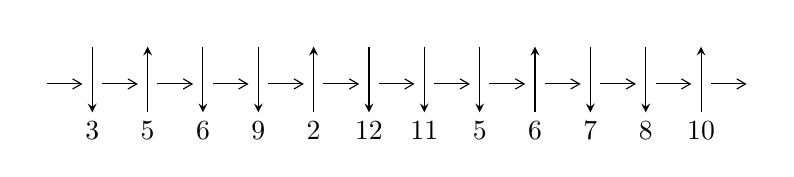
\begin{tikzpicture}[x=20pt, y=17pt]
	% nodes
	\node (C0) at (0, 0) {};
	\node (C1) at (1, 0) {};
	\node (C1U) at (1, +1) {};
	\node (C1D) at (1, -1) {3};

	\node (C2) at (2, 0) {};
	\node (C2U) at (2, +1) {};
	\node (C2D) at (2, -1) {5};

	\node (C3) at (3, 0) {};
	\node (C3U) at (3, +1) {};
	\node (C3D) at (3, -1) {6};

	\node (C4) at (4, 0) {};
	\node (C4U) at (4, +1) {};
	\node (C4D) at (4, -1) {9};

	\node (C5) at (5, 0) {};
	\node (C5U) at (5, +1) {};
	\node (C5D) at (5, -1) {2};

	\node (C6) at (6, 0) {};
	\node (C6U) at (6, +1) {};
	\node (C6D) at (6, -1) {12};

	\node (C7) at (7, 0) {};
	\node (C7U) at (7, +1) {};
	\node (C7D) at (7, -1) {11};

	\node (C8) at (8, 0) {};
	\node (C8U) at (8, +1) {};
	\node (C8D) at (8, -1) {5};

	\node (C9) at (9, 0) {};
	\node (C9U) at (9, +1) {};
	\node (C9D) at (9, -1) {6};

	\node (C10) at (10, 0) {};
	\node (C10U) at (10, +1) {};
	\node (C10D) at (10, -1) {7};

	\node (C11) at (11, 0) {};
	\node (C11U) at (11, +1) {};
	\node (C11D) at (11, -1) {8};

	\node (C12) at (12, 0) {};
	\node (C12U) at (12, +1) {};
	\node (C12D) at (12, -1) {10};
	\node (C13) at (13, 0) {};

	% arrows
	\draw[->,>={angle 60}]
	(C0) edge (C1) (C1) edge (C2) (C2) edge (C3) (C3) edge (C4) (C4) edge (C5) (C5) edge (C6) (C6) edge (C7) (C7) edge (C8) (C8) edge (C9) (C9) edge (C10) (C10) edge (C11) (C11) edge (C12) (C12) edge (C13) ;	\draw[->,>=stealth]
	(C1U) edge (C1D) (C2D) edge (C2U) (C3U) edge (C3D) (C4U) edge (C4D) (C5D) edge (C5U) (C6U) edge (C6D) (C7U) edge (C7D) (C8U) edge (C8D) (C9D) edge (C9U) (C10U) edge (C10D) (C11U) edge (C11D) (C12D) edge (C12U) ;
	\end{tikzpicture} \\
\hhline{~~} \\& 
\textbf{Solving Sequence} \\ \cline{2-2} 
 &
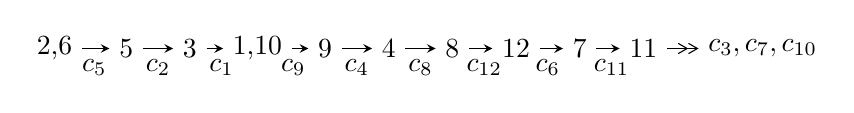
\begin{tikzpicture}[x=23pt, y=7pt]
	% node
	\node (A0) at (-1/8, 0) {2,6};
	\node (A1) at (1, 0) {5};
	\node (A2) at (2, 0) {3};
	\node (A3) at (49/16, 0) {1,10};
	\node (A4) at (33/8, 0) {9};
	\node (A5) at (41/8, 0) {4};
	\node (A6) at (49/8, 0) {8};
	\node (A7) at (57/8, 0) {12};
	\node (A8) at (65/8, 0) {7};
	\node (A9) at (73/8, 0) {11};
	\node (C1) at (1/2, -1) {$c_{5}$};
	\node (C2) at (3/2, -1) {$c_{2}$};
	\node (C3) at (5/2, -1) {$c_{1}$};
	\node (C4) at (29/8, -1) {$c_{9}$};
	\node (C5) at (37/8, -1) {$c_{4}$};
	\node (C6) at (45/8, -1) {$c_{8}$};
	\node (C7) at (53/8, -1) {$c_{12}$};
	\node (C8) at (61/8, -1) {$c_{6}$};
	\node (C9) at (69/8, -1) {$c_{11}$};
	\node (A10) at (11, 0) {$c_{3},c_{7},c_{10}$};

	% edge
	\draw[->,>=stealth]	
	(A0) edge (A1) (A1) edge (A2) (A2) edge (A3) (A3) edge (A4) (A4) edge (A5) (A5) edge (A6) (A6) edge (A7) (A7) edge (A8) (A8) edge (A9) ;
	\draw[->>,>={angle 60}]	
	(A9) edge (A10);
\end{tikzpicture} \\ 

\end{tabular} \\

\footnotetext{
The image of knot diagram is generated by the software ``\textbf{Draw programme}" developed by Andrew Bartholomew(\url{http://www.layer8.co.uk/maths/draw/index.htm\#Running-draw}), where we modified some parts for our purpose(\url{https://github.com/CATsTAILs/LinksPainter}).
}\phantom \\ \newline 
\centering \textbf{Ideals for irreducible components\footnotemark of $X_{\text{par}}$} 
 
\begin{align*}
I^u_{1}&=\langle 
18 u^{38}+107 u^{37}+\cdots+16 b-35,\;-35 u^{38}-228 u^{37}+\cdots+16 a-167,\;u^{39}+6 u^{38}+\cdots+6 u+1\rangle \\
I^u_{2}&=\langle 
- a u+b,\;a^5+a^4 u- a^4-2 a^3 u+a^2+a u- a- u,\;u^2- u+1\rangle \\
\\
\end{align*}
\raggedright * 2 irreducible components of $\dim_{\mathbb{C}}=0$, with total 49 representations.\\
\footnotetext{All coefficients of polynomials are rational numbers. But the coefficients are sometimes approximated in decimal forms when there is not enough margin.}
\newpage
\renewcommand{\arraystretch}{1}
\centering \section*{I. $I^u_{1}= \langle 18 u^{38}+107 u^{37}+\cdots+16 b-35,\;-35 u^{38}-228 u^{37}+\cdots+16 a-167,\;u^{39}+6 u^{38}+\cdots+6 u+1 \rangle$}
\flushleft \textbf{(i) Arc colorings}\\
\begin{tabular}{m{7pt} m{180pt} m{7pt} m{180pt} }
\flushright $a_{2}=$&$\begin{pmatrix}0\\u\end{pmatrix}$ \\
\flushright $a_{6}=$&$\begin{pmatrix}1\\0\end{pmatrix}$ \\
\flushright $a_{5}=$&$\begin{pmatrix}1\\u^2\end{pmatrix}$ \\
\flushright $a_{3}=$&$\begin{pmatrix}u\\u^3+u\end{pmatrix}$ \\
\flushright $a_{1}=$&$\begin{pmatrix}u^3\\u^5+u^3+u\end{pmatrix}$ \\
\flushright $a_{10}=$&$\begin{pmatrix}2.18750 u^{38}+14.2500 u^{37}+\cdots+54.5000 u+10.4375\\-1.12500 u^{38}-6.68750 u^{37}+\cdots+2.68750 u+2.18750\end{pmatrix}$ \\
\flushright $a_{9}=$&$\begin{pmatrix}3.31250 u^{38}+20.9375 u^{37}+\cdots+51.8125 u+8.25000\\-1.12500 u^{38}-6.68750 u^{37}+\cdots+2.68750 u+2.18750\end{pmatrix}$ \\
\flushright $a_{4}=$&$\begin{pmatrix}- u^3\\u^3+u\end{pmatrix}$ \\
\flushright $a_{8}=$&$\begin{pmatrix}3.18750 u^{38}+21.3125 u^{37}+\cdots+64.1875 u+11.5000\\-3.12500 u^{38}-15.5625 u^{37}+\cdots-3.93750 u+1.06250\end{pmatrix}$ \\
\flushright $a_{12}=$&$\begin{pmatrix}-0.0625000 u^{37}-0.312500 u^{36}+\cdots-2.31250 u+0.937500\\0.0625000 u^{38}+0.312500 u^{37}+\cdots+2.31250 u^{2}+0.0625000 u\end{pmatrix}$ \\
\flushright $a_{7}=$&$\begin{pmatrix}0.875000 u^{38}+5.18750 u^{37}+\cdots+5.56250 u+1.93750\\0.687500 u^{37}+3.43750 u^{36}+\cdots+3.93750 u+0.812500\end{pmatrix}$ \\
\flushright $a_{11}=$&$\begin{pmatrix}-\frac{3}{4} u^{38}-4 u^{37}+\cdots-\frac{17}{8} u-\frac{1}{4}\\\frac{1}{8} u^{38}+\frac{1}{16} u^{37}+\cdots-\frac{35}{16} u-\frac{11}{16}\end{pmatrix}$\\&\end{tabular}
\flushleft \textbf{(ii) Obstruction class $= -1$}\\~\\
\flushleft \textbf{(iii) Cusp Shapes $= \frac{227}{16} u^{38}+\frac{1349}{16} u^{37}+\cdots+\frac{1989}{16} u+\frac{25}{2}$}\\~\\
\newpage\renewcommand{\arraystretch}{1}
\flushleft \textbf{(iv) u-Polynomials at the component}\newline \\
\begin{tabular}{m{50pt}|m{274pt}}
Crossings & \hspace{64pt}u-Polynomials at each crossing \\
\hline $$\begin{aligned}c_{1}\end{aligned}$$&$\begin{aligned}
&u^{39}+8 u^{38}+\cdots-10 u-1
\end{aligned}$\\
\hline $$\begin{aligned}c_{2},c_{5}\end{aligned}$$&$\begin{aligned}
&u^{39}+6 u^{38}+\cdots+6 u+1
\end{aligned}$\\
\hline $$\begin{aligned}c_{3}\end{aligned}$$&$\begin{aligned}
&u^{39}-6 u^{38}+\cdots+227832 u+23497
\end{aligned}$\\
\hline $$\begin{aligned}c_{4},c_{8}\end{aligned}$$&$\begin{aligned}
&u^{39}+u^{38}+\cdots+2048 u+1024
\end{aligned}$\\
\hline $$\begin{aligned}c_{6}\end{aligned}$$&$\begin{aligned}
&u^{39}-9 u^{38}+\cdots+179 u-17
\end{aligned}$\\
\hline $$\begin{aligned}c_{7},c_{10},c_{11}\end{aligned}$$&$\begin{aligned}
&u^{39}+3 u^{38}+\cdots-3 u+1
\end{aligned}$\\
\hline $$\begin{aligned}c_{9}\end{aligned}$$&$\begin{aligned}
&u^{39}-3 u^{38}+\cdots-3 u+1
\end{aligned}$\\
\hline $$\begin{aligned}c_{12}\end{aligned}$$&$\begin{aligned}
&u^{39}+11 u^{38}+\cdots+267 u+73
\end{aligned}$\\
\hline
\end{tabular}\\~\\
\newpage\renewcommand{\arraystretch}{1}
\flushleft \textbf{(v) Riley Polynomials at the component}\newline \\
\begin{tabular}{m{50pt}|m{274pt}}
Crossings & \hspace{64pt}Riley Polynomials at each crossing \\
\hline $$\begin{aligned}c_{1}\end{aligned}$$&$\begin{aligned}
&y^{39}+52 y^{38}+\cdots+58 y-1
\end{aligned}$\\
\hline $$\begin{aligned}c_{2},c_{5}\end{aligned}$$&$\begin{aligned}
&y^{39}+8 y^{38}+\cdots-10 y-1
\end{aligned}$\\
\hline $$\begin{aligned}c_{3}\end{aligned}$$&$\begin{aligned}
&y^{39}+96 y^{38}+\cdots-14329729890 y-552109009
\end{aligned}$\\
\hline $$\begin{aligned}c_{4},c_{8}\end{aligned}$$&$\begin{aligned}
&y^{39}+55 y^{38}+\cdots-5242880 y-1048576
\end{aligned}$\\
\hline $$\begin{aligned}c_{6}\end{aligned}$$&$\begin{aligned}
&y^{39}+9 y^{38}+\cdots+2665 y-289
\end{aligned}$\\
\hline $$\begin{aligned}c_{7},c_{10},c_{11}\end{aligned}$$&$\begin{aligned}
&y^{39}-35 y^{38}+\cdots-3 y-1
\end{aligned}$\\
\hline $$\begin{aligned}c_{9}\end{aligned}$$&$\begin{aligned}
&y^{39}-67 y^{38}+\cdots-3 y-1
\end{aligned}$\\
\hline $$\begin{aligned}c_{12}\end{aligned}$$&$\begin{aligned}
&y^{39}-7 y^{38}+\cdots-292543 y-5329
\end{aligned}$\\
\hline
\end{tabular}\\~\\
\newpage\flushleft \textbf{(vi) Complex Volumes and Cusp Shapes}
$$\begin{array}{c|c|c}  
\text{Solutions to }I^u_{1}& \I (\text{vol} + \sqrt{-1}CS) & \text{Cusp shape}\\
 \hline 
\begin{aligned}
u &= \phantom{-}0.217775 + 0.986965 I \\
a &= \phantom{-}0.478937 - 0.405328 I \\
b &= -0.504345 - 0.384424 I\end{aligned}
 & -5.08086 + 0.15570 I & -9.83989 - 1.69370 I \\ \hline\begin{aligned}
u &= \phantom{-}0.217775 - 0.986965 I \\
a &= \phantom{-}0.478937 + 0.405328 I \\
b &= -0.504345 + 0.384424 I\end{aligned}
 & -5.08086 - 0.15570 I & -9.83989 + 1.69370 I \\ \hline\begin{aligned}
u &= \phantom{-}0.795838 + 0.548145 I \\
a &= \phantom{-}0.160432 + 0.477438 I \\
b &= \phantom{-}0.134027 - 0.467904 I\end{aligned}
 & \phantom{-}2.99441 + 1.56903 I & \phantom{-}2.04971 - 2.63058 I \\ \hline\begin{aligned}
u &= \phantom{-}0.795838 - 0.548145 I \\
a &= \phantom{-}0.160432 - 0.477438 I \\
b &= \phantom{-}0.134027 + 0.467904 I\end{aligned}
 & \phantom{-}2.99441 - 1.56903 I & \phantom{-}2.04971 + 2.63058 I \\ \hline\begin{aligned}
u &= \phantom{-}0.395368 + 0.848396 I \\
a &= -0.328402 + 0.067571 I \\
b &= \phantom{-}0.187167 + 0.251900 I\end{aligned}
 & -0.32291 + 1.65676 I & -2.57784 - 5.09388 I \\ \hline\begin{aligned}
u &= \phantom{-}0.395368 - 0.848396 I \\
a &= -0.328402 - 0.067571 I \\
b &= \phantom{-}0.187167 - 0.251900 I\end{aligned}
 & -0.32291 - 1.65676 I & -2.57784 + 5.09388 I \\ \hline\begin{aligned}
u &= \phantom{-}0.835550 + 0.682012 I \\
a &= -0.122808 - 0.434535 I \\
b &= -0.193746 + 0.446832 I\end{aligned}
 & -1.08176 + 5.00495 I & -4.00000 - 5.49460 I \\ \hline\begin{aligned}
u &= \phantom{-}0.835550 - 0.682012 I \\
a &= -0.122808 + 0.434535 I \\
b &= -0.193746 - 0.446832 I\end{aligned}
 & -1.08176 - 5.00495 I & -4.00000 + 5.49460 I \\ \hline\begin{aligned}
u &= \phantom{-}0.820354 + 0.374203 I \\
a &= -0.141671 - 0.553737 I \\
b &= -0.090989 + 0.507274 I\end{aligned}
 & -0.79445 - 1.82967 I & -2.60045 + 1.37386 I \\ \hline\begin{aligned}
u &= \phantom{-}0.820354 - 0.374203 I \\
a &= -0.141671 + 0.553737 I \\
b &= -0.090989 - 0.507274 I\end{aligned}
 & -0.79445 + 1.82967 I & -2.60045 - 1.37386 I\\
 \hline 
 \end{array}$$\newpage$$\begin{array}{c|c|c}  
\text{Solutions to }I^u_{1}& \I (\text{vol} + \sqrt{-1}CS) & \text{Cusp shape}\\
 \hline 
\begin{aligned}
u &= \phantom{-}0.516539 + 1.059320 I \\
a &= \phantom{-}0.121118 - 0.354987 I \\
b &= -0.438608 + 0.055062 I\end{aligned}
 & \phantom{-}1.18484 + 3.42225 I & \phantom{-0.000000 } 0. - 3.84715 I \\ \hline\begin{aligned}
u &= \phantom{-}0.516539 - 1.059320 I \\
a &= \phantom{-}0.121118 + 0.354987 I \\
b &= -0.438608 - 0.055062 I\end{aligned}
 & \phantom{-}1.18484 - 3.42225 I & \phantom{-0.000000 -}0. + 3.84715 I \\ \hline\begin{aligned}
u &= \phantom{-}0.639199 + 1.006420 I \\
a &= -0.023637 + 0.351005 I \\
b &= \phantom{-}0.368368 - 0.200573 I\end{aligned}
 & -2.22349 + 0.53849 I & -5.53531 + 1.24212 I \\ \hline\begin{aligned}
u &= \phantom{-}0.639199 - 1.006420 I \\
a &= -0.023637 - 0.351005 I \\
b &= \phantom{-}0.368368 + 0.200573 I\end{aligned}
 & -2.22349 - 0.53849 I & -5.53531 - 1.24212 I \\ \hline\begin{aligned}
u &= \phantom{-}0.463738 + 1.131070 I \\
a &= -0.157364 + 0.415273 I \\
b &= \phantom{-}0.542679 - 0.014588 I\end{aligned}
 & -3.39936 + 6.68540 I & -5.94355 - 5.90487 I \\ \hline\begin{aligned}
u &= \phantom{-}0.463738 - 1.131070 I \\
a &= -0.157364 - 0.415273 I \\
b &= \phantom{-}0.542679 + 0.014588 I\end{aligned}
 & -3.39936 - 6.68540 I & -5.94355 + 5.90487 I \\ \hline\begin{aligned}
u &= -0.146263 + 0.696408 I \\
a &= \phantom{-}1.54768 - 0.36171 I \\
b &= -0.025530 - 1.130720 I\end{aligned}
 & -6.52633 + 3.36713 I & -11.83061 - 4.84786 I \\ \hline\begin{aligned}
u &= -0.146263 - 0.696408 I \\
a &= \phantom{-}1.54768 + 0.36171 I \\
b &= -0.025530 + 1.130720 I\end{aligned}
 & -6.52633 - 3.36713 I & -11.83061 + 4.84786 I \\ \hline\begin{aligned}
u &= -0.887416 + 0.936488 I \\
a &= -1.41323 - 1.17323 I \\
b &= -2.35284 + 0.28232 I\end{aligned}
 & \phantom{-}2.09421 - 3.28881 I & \phantom{-0.000000 } 0 \\ \hline\begin{aligned}
u &= -0.887416 - 0.936488 I \\
a &= -1.41323 + 1.17323 I \\
b &= -2.35284 - 0.28232 I\end{aligned}
 & \phantom{-}2.09421 + 3.28881 I & \phantom{-0.000000 } 0\\
 \hline 
 \end{array}$$\newpage$$\begin{array}{c|c|c}  
\text{Solutions to }I^u_{1}& \I (\text{vol} + \sqrt{-1}CS) & \text{Cusp shape}\\
 \hline 
\begin{aligned}
u &= -1.018770 + 0.851930 I \\
a &= \phantom{-}1.42653 + 0.88370 I \\
b &= \phantom{-}2.20615 - 0.31501 I\end{aligned}
 & \phantom{-}7.27711 + 5.72796 I & \phantom{-0.000000 } 0 \\ \hline\begin{aligned}
u &= -1.018770 - 0.851930 I \\
a &= \phantom{-}1.42653 - 0.88370 I \\
b &= \phantom{-}2.20615 + 0.31501 I\end{aligned}
 & \phantom{-}7.27711 - 5.72796 I & \phantom{-0.000000 } 0 \\ \hline\begin{aligned}
u &= -1.012200 + 0.890886 I \\
a &= -1.38271 - 0.92662 I \\
b &= -2.22509 + 0.29392 I\end{aligned}
 & \phantom{-}12.39950 + 1.53189 I & \phantom{-0.000000 } 0 \\ \hline\begin{aligned}
u &= -1.012200 - 0.890886 I \\
a &= -1.38271 + 0.92662 I \\
b &= -2.22509 - 0.29392 I\end{aligned}
 & \phantom{-}12.39950 - 1.53189 I & \phantom{-0.000000 } 0 \\ \hline\begin{aligned}
u &= -0.364738 + 0.539930 I \\
a &= -2.16669 - 0.02235 I \\
b &= -0.802344 + 1.161710 I\end{aligned}
 & -5.82107 - 5.39582 I & -8.47886 + 1.18765 I \\ \hline\begin{aligned}
u &= -0.364738 - 0.539930 I \\
a &= -2.16669 + 0.02235 I \\
b &= -0.802344 - 1.161710 I\end{aligned}
 & -5.82107 + 5.39582 I & -8.47886 - 1.18765 I \\ \hline\begin{aligned}
u &= -0.985908 + 0.935010 I \\
a &= \phantom{-}1.34032 + 0.99776 I \\
b &= \phantom{-}2.25434 - 0.26951 I\end{aligned}
 & \phantom{-}10.13770 - 2.96345 I & \phantom{-0.000000 } 0 \\ \hline\begin{aligned}
u &= -0.985908 - 0.935010 I \\
a &= \phantom{-}1.34032 - 0.99776 I \\
b &= \phantom{-}2.25434 + 0.26951 I\end{aligned}
 & \phantom{-}10.13770 + 2.96345 I & \phantom{-0.000000 } 0 \\ \hline\begin{aligned}
u &= -0.939008 + 1.004180 I \\
a &= \phantom{-}1.25206 + 1.11303 I \\
b &= \phantom{-}2.29337 - 0.21215 I\end{aligned}
 & \phantom{-}9.89948 - 4.09070 I & \phantom{-0.000000 } 0 \\ \hline\begin{aligned}
u &= -0.939008 - 1.004180 I \\
a &= \phantom{-}1.25206 - 1.11303 I \\
b &= \phantom{-}2.29337 + 0.21215 I\end{aligned}
 & \phantom{-}9.89948 + 4.09070 I & \phantom{-0.000000 } 0\\
 \hline 
 \end{array}$$\newpage$$\begin{array}{c|c|c}  
\text{Solutions to }I^u_{1}& \I (\text{vol} + \sqrt{-1}CS) & \text{Cusp shape}\\
 \hline 
\begin{aligned}
u &= -0.894077 + 1.060480 I \\
a &= \phantom{-}1.15539 + 1.20734 I \\
b &= \phantom{-}2.31337 - 0.14581 I\end{aligned}
 & \phantom{-}6.5826 - 12.7219 I & \phantom{-0.000000 } 0 \\ \hline\begin{aligned}
u &= -0.894077 - 1.060480 I \\
a &= \phantom{-}1.15539 - 1.20734 I \\
b &= \phantom{-}2.31337 + 0.14581 I\end{aligned}
 & \phantom{-}6.5826 + 12.7219 I & \phantom{-0.000000 } 0 \\ \hline\begin{aligned}
u &= -0.918184 + 1.042580 I \\
a &= -1.18777 - 1.16067 I \\
b &= -2.30068 + 0.17262 I\end{aligned}
 & \phantom{-}11.8898 - 8.5952 I & \phantom{-0.000000 } 0 \\ \hline\begin{aligned}
u &= -0.918184 - 1.042580 I \\
a &= -1.18777 + 1.16067 I \\
b &= -2.30068 - 0.17262 I\end{aligned}
 & \phantom{-}11.8898 + 8.5952 I & \phantom{-0.000000 } 0 \\ \hline\begin{aligned}
u &= -0.304253 + 0.441278 I \\
a &= \phantom{-}2.04672 + 0.15438 I \\
b &= \phantom{-}0.690845 - 0.856203 I\end{aligned}
 & -0.29697 - 2.23720 I & -4.18982 + 2.52656 I \\ \hline\begin{aligned}
u &= -0.304253 - 0.441278 I \\
a &= \phantom{-}2.04672 - 0.15438 I \\
b &= \phantom{-}0.690845 + 0.856203 I\end{aligned}
 & -0.29697 + 2.23720 I & -4.18982 - 2.52656 I \\ \hline\begin{aligned}
u &= -0.035517 + 0.529752 I \\
a &= -1.44264 - 0.17191 I \\
b &= -0.142307 + 0.758134 I\end{aligned}
 & -0.933124 + 0.964799 I & -7.52834 - 5.01190 I \\ \hline\begin{aligned}
u &= -0.035517 - 0.529752 I \\
a &= -1.44264 + 0.17191 I \\
b &= -0.142307 - 0.758134 I\end{aligned}
 & -0.933124 - 0.964799 I & -7.52834 + 5.01190 I \\ \hline\begin{aligned}
u &= -0.356068\phantom{ +0.000000I} \\
a &= -2.32453\phantom{ +0.000000I} \\
b &= -0.827691\phantom{ +0.000000I}\end{aligned}
 & -1.93664\phantom{ +0.000000I} & -5.10000\phantom{ +0.000000I}\\
 \hline 
 \end{array}$$\newpage\newpage\renewcommand{\arraystretch}{1}
\centering \section*{II. $I^u_{2}= \langle - a u+b,\;a^5+a^4 u- a^4-2 a^3 u+a^2+a u- a- u,\;u^2- u+1 \rangle$}
\flushleft \textbf{(i) Arc colorings}\\
\begin{tabular}{m{7pt} m{180pt} m{7pt} m{180pt} }
\flushright $a_{2}=$&$\begin{pmatrix}0\\u\end{pmatrix}$ \\
\flushright $a_{6}=$&$\begin{pmatrix}1\\0\end{pmatrix}$ \\
\flushright $a_{5}=$&$\begin{pmatrix}1\\u-1\end{pmatrix}$ \\
\flushright $a_{3}=$&$\begin{pmatrix}u\\u-1\end{pmatrix}$ \\
\flushright $a_{1}=$&$\begin{pmatrix}-1\\0\end{pmatrix}$ \\
\flushright $a_{10}=$&$\begin{pmatrix}a\\a u\end{pmatrix}$ \\
\flushright $a_{9}=$&$\begin{pmatrix}- a u+a\\a u\end{pmatrix}$ \\
\flushright $a_{4}=$&$\begin{pmatrix}1\\u-1\end{pmatrix}$ \\
\flushright $a_{8}=$&$\begin{pmatrix}- a u+a\\a u\end{pmatrix}$ \\
\flushright $a_{12}=$&$\begin{pmatrix}- a^2 u-1\\- a^2 u+a^2\end{pmatrix}$ \\
\flushright $a_{7}=$&$\begin{pmatrix}- a^4+a^2 u- a^2+1\\- a^4 u\end{pmatrix}$ \\
\flushright $a_{11}=$&$\begin{pmatrix}a^4 u- a^4- a^2 u+a^2-1\\- a^4 u\end{pmatrix}$\\&\end{tabular}
\flushleft \textbf{(ii) Obstruction class $= 1$}\\~\\
\flushleft \textbf{(iii) Cusp Shapes $= a^4 u- a^4-4 a^3-5 a^2 u+5 a^2+3 a u+a-4 u-6$}\\~\\
\newpage\renewcommand{\arraystretch}{1}
\flushleft \textbf{(iv) u-Polynomials at the component}\newline \\
\begin{tabular}{m{50pt}|m{274pt}}
Crossings & \hspace{64pt}u-Polynomials at each crossing \\
\hline $$\begin{aligned}c_{1},c_{3},c_{5}\end{aligned}$$&$\begin{aligned}
&(u^2- u+1)^5
\end{aligned}$\\
\hline $$\begin{aligned}c_{2}\end{aligned}$$&$\begin{aligned}
&(u^2+u+1)^5
\end{aligned}$\\
\hline $$\begin{aligned}c_{4},c_{8}\end{aligned}$$&$\begin{aligned}
&u^{10}
\end{aligned}$\\
\hline $$\begin{aligned}c_{6}\end{aligned}$$&$\begin{aligned}
&(u^5-3 u^4+4 u^3- u^2- u+1)^2
\end{aligned}$\\
\hline $$\begin{aligned}c_{7}\end{aligned}$$&$\begin{aligned}
&(u^5+u^4-2 u^3- u^2+u-1)^2
\end{aligned}$\\
\hline $$\begin{aligned}c_{9},c_{12}\end{aligned}$$&$\begin{aligned}
&(u^5+u^4+2 u^3+u^2+u+1)^2
\end{aligned}$\\
\hline $$\begin{aligned}c_{10},c_{11}\end{aligned}$$&$\begin{aligned}
&(u^5- u^4-2 u^3+u^2+u+1)^2
\end{aligned}$\\
\hline
\end{tabular}\\~\\
\newpage\renewcommand{\arraystretch}{1}
\flushleft \textbf{(v) Riley Polynomials at the component}\newline \\
\begin{tabular}{m{50pt}|m{274pt}}
Crossings & \hspace{64pt}Riley Polynomials at each crossing \\
\hline $$\begin{aligned}c_{1},c_{2},c_{3}\\c_{5}\end{aligned}$$&$\begin{aligned}
&(y^2+y+1)^5
\end{aligned}$\\
\hline $$\begin{aligned}c_{4},c_{8}\end{aligned}$$&$\begin{aligned}
&y^{10}
\end{aligned}$\\
\hline $$\begin{aligned}c_{6}\end{aligned}$$&$\begin{aligned}
&(y^5- y^4+8 y^3-3 y^2+3 y-1)^2
\end{aligned}$\\
\hline $$\begin{aligned}c_{7},c_{10},c_{11}\end{aligned}$$&$\begin{aligned}
&(y^5-5 y^4+8 y^3-3 y^2- y-1)^2
\end{aligned}$\\
\hline $$\begin{aligned}c_{9},c_{12}\end{aligned}$$&$\begin{aligned}
&(y^5+3 y^4+4 y^3+y^2- y-1)^2
\end{aligned}$\\
\hline
\end{tabular}\\~\\
\newpage\flushleft \textbf{(vi) Complex Volumes and Cusp Shapes}
$$\begin{array}{c|c|c}  
\text{Solutions to }I^u_{2}& \I (\text{vol} + \sqrt{-1}CS) & \text{Cusp shape}\\
 \hline 
\begin{aligned}
u &= \phantom{-}0.500000 + 0.866025 I \\
a &= -0.881753 - 0.117510 I \\
b &= -0.339110 - 0.822375 I\end{aligned}
 & -0.329100 + 0.499304 I & -2.53179 + 1.09027 I \\ \hline\begin{aligned}
u &= \phantom{-}0.500000 + 0.866025 I \\
a &= \phantom{-}0.542643 + 0.704866 I \\
b &= -0.339110 + 0.822375 I\end{aligned}
 & -0.32910 + 3.56046 I & -5.04069 - 7.43801 I \\ \hline\begin{aligned}
u &= \phantom{-}0.500000 + 0.866025 I \\
a &= \phantom{-}0.383413 - 0.664091 I \\
b &= \phantom{-}0.766826\phantom{ +0.000000I}\end{aligned}
 & -2.40108 + 2.02988 I & -6.62546 - 4.42764 I \\ \hline\begin{aligned}
u &= \phantom{-}0.500000 + 0.866025 I \\
a &= -0.811514 - 0.994721 I \\
b &= \phantom{-}0.455697 - 1.200150 I\end{aligned}
 & -5.87256 - 2.37095 I & -6.60498 - 0.29447 I \\ \hline\begin{aligned}
u &= \phantom{-}0.500000 + 0.866025 I \\
a &= \phantom{-}1.267210 + 0.205431 I \\
b &= \phantom{-}0.455697 + 1.200150 I\end{aligned}
 & -5.87256 + 6.43072 I & -9.19707 - 7.98272 I \\ \hline\begin{aligned}
u &= \phantom{-}0.500000 - 0.866025 I \\
a &= -0.881753 + 0.117510 I \\
b &= -0.339110 + 0.822375 I\end{aligned}
 & -0.329100 - 0.499304 I & -2.53179 - 1.09027 I \\ \hline\begin{aligned}
u &= \phantom{-}0.500000 - 0.866025 I \\
a &= \phantom{-}0.542643 - 0.704866 I \\
b &= -0.339110 - 0.822375 I\end{aligned}
 & -0.32910 - 3.56046 I & -5.04069 + 7.43801 I \\ \hline\begin{aligned}
u &= \phantom{-}0.500000 - 0.866025 I \\
a &= \phantom{-}0.383413 + 0.664091 I \\
b &= \phantom{-}0.766826\phantom{ +0.000000I}\end{aligned}
 & -2.40108 - 2.02988 I & -6.62546 + 4.42764 I \\ \hline\begin{aligned}
u &= \phantom{-}0.500000 - 0.866025 I \\
a &= -0.811514 + 0.994721 I \\
b &= \phantom{-}0.455697 + 1.200150 I\end{aligned}
 & -5.87256 + 2.37095 I & -6.60498 + 0.29447 I \\ \hline\begin{aligned}
u &= \phantom{-}0.500000 - 0.866025 I \\
a &= \phantom{-}1.267210 - 0.205431 I \\
b &= \phantom{-}0.455697 - 1.200150 I\end{aligned}
 & -5.87256 - 6.43072 I & -9.19707 + 7.98272 I\\
 \hline 
 \end{array}$$\newpage
\newpage\renewcommand{\arraystretch}{1}
\centering \section*{ III. u-Polynomials}
\begin{tabular}{m{50pt}|m{274pt}}
Crossings & \hspace{64pt}u-Polynomials at each crossing \\
\hline $$\begin{aligned}c_{1}\end{aligned}$$&$\begin{aligned}
&((u^2- u+1)^5)(u^{39}+8 u^{38}+\cdots-10 u-1)
\end{aligned}$\\
\hline $$\begin{aligned}c_{2}\end{aligned}$$&$\begin{aligned}
&((u^2+u+1)^5)(u^{39}+6 u^{38}+\cdots+6 u+1)
\end{aligned}$\\
\hline $$\begin{aligned}c_{3}\end{aligned}$$&$\begin{aligned}
&((u^2- u+1)^5)(u^{39}-6 u^{38}+\cdots+227832 u+23497)
\end{aligned}$\\
\hline $$\begin{aligned}c_{4},c_{8}\end{aligned}$$&$\begin{aligned}
&u^{10}(u^{39}+u^{38}+\cdots+2048 u+1024)
\end{aligned}$\\
\hline $$\begin{aligned}c_{5}\end{aligned}$$&$\begin{aligned}
&((u^2- u+1)^5)(u^{39}+6 u^{38}+\cdots+6 u+1)
\end{aligned}$\\
\hline $$\begin{aligned}c_{6}\end{aligned}$$&$\begin{aligned}
&((u^5-3 u^4+4 u^3- u^2- u+1)^2)(u^{39}-9 u^{38}+\cdots+179 u-17)
\end{aligned}$\\
\hline $$\begin{aligned}c_{7}\end{aligned}$$&$\begin{aligned}
&((u^5+u^4-2 u^3- u^2+u-1)^2)(u^{39}+3 u^{38}+\cdots-3 u+1)
\end{aligned}$\\
\hline $$\begin{aligned}c_{9}\end{aligned}$$&$\begin{aligned}
&((u^5+u^4+2 u^3+u^2+u+1)^2)(u^{39}-3 u^{38}+\cdots-3 u+1)
\end{aligned}$\\
\hline $$\begin{aligned}c_{10},c_{11}\end{aligned}$$&$\begin{aligned}
&((u^5- u^4-2 u^3+u^2+u+1)^2)(u^{39}+3 u^{38}+\cdots-3 u+1)
\end{aligned}$\\
\hline $$\begin{aligned}c_{12}\end{aligned}$$&$\begin{aligned}
&((u^5+u^4+2 u^3+u^2+u+1)^2)(u^{39}+11 u^{38}+\cdots+267 u+73)
\end{aligned}$\\
\hline
\end{tabular}\newpage\renewcommand{\arraystretch}{1}
\centering \section*{ IV. Riley Polynomials}
\begin{tabular}{m{50pt}|m{274pt}}
Crossings & \hspace{64pt}Riley Polynomials at each crossing \\
\hline $$\begin{aligned}c_{1}\end{aligned}$$&$\begin{aligned}
&((y^2+y+1)^5)(y^{39}+52 y^{38}+\cdots+58 y-1)
\end{aligned}$\\
\hline $$\begin{aligned}c_{2},c_{5}\end{aligned}$$&$\begin{aligned}
&((y^2+y+1)^5)(y^{39}+8 y^{38}+\cdots-10 y-1)
\end{aligned}$\\
\hline $$\begin{aligned}c_{3}\end{aligned}$$&$\begin{aligned}
&((y^2+y+1)^5)(y^{39}+96 y^{38}+\cdots-1.43297\times10^{10} y-5.52109\times10^{8})
\end{aligned}$\\
\hline $$\begin{aligned}c_{4},c_{8}\end{aligned}$$&$\begin{aligned}
&y^{10}(y^{39}+55 y^{38}+\cdots-5242880 y-1048576)
\end{aligned}$\\
\hline $$\begin{aligned}c_{6}\end{aligned}$$&$\begin{aligned}
&((y^5- y^4+8 y^3-3 y^2+3 y-1)^2)(y^{39}+9 y^{38}+\cdots+2665 y-289)
\end{aligned}$\\
\hline $$\begin{aligned}c_{7},c_{10},c_{11}\end{aligned}$$&$\begin{aligned}
&((y^5-5 y^4+8 y^3-3 y^2- y-1)^2)(y^{39}-35 y^{38}+\cdots-3 y-1)
\end{aligned}$\\
\hline $$\begin{aligned}c_{9}\end{aligned}$$&$\begin{aligned}
&((y^5+3 y^4+4 y^3+y^2- y-1)^2)(y^{39}-67 y^{38}+\cdots-3 y-1)
\end{aligned}$\\
\hline $$\begin{aligned}c_{12}\end{aligned}$$&$\begin{aligned}
&((y^5+3 y^4+4 y^3+y^2- y-1)^2)(y^{39}-7 y^{38}+\cdots-292543 y-5329)
\end{aligned}$\\
\hline
\end{tabular}
\vskip 2pc
\end{document}